\documentclass[10pt]{article}
\usepackage{array, xcolor, lipsum, bibentry}
\usepackage[margin=1.2cm]{geometry}
\usepackage{multicol}
\usepackage{setspace}
\usepackage{paralist}


\ifx\pdftexversion\undefined
 \usepackage[dvips]{graphicx}
 \else
 
 \usepackage[pdftex]{graphicx}
 \DeclareGraphicsRule{*}{mps}{*}{}
 \fi
\title{\bfseries\Huge Aneesh Kumar}
\author{anush0247@gmail.com}
\date{}
 
\definecolor{lightgray}{gray}{0.6}
\newcolumntype{L}{>{\raggedleft}p{0.14\textwidth}}
\newcolumntype{R}{p{0.8\textwidth}}
\newcommand\VRule{\color{lightgray}\vrule width 1pt}
 

\begin{document}
\fontfamily{cmr}
\pagestyle{empty}
\begin{center}
\Large
\textbf{Curriculum Vitae}
\end{center}
\normalsize
\begin{multicols}{2}
\paragraph{\large Aneesh Kumar Thangella}
\normalsize	
 \url{\\ 20 Years, Male \\
 N090247, 4th Year B.Tech CSE\\
 RGUKT Nuzvid, Krishna Dt., A.P. - India 
}
\begin{flushright}
\underline{} \\

 \url{+91 9160883374} \\
 \url{anush0247@gmail.com} \\
 \url{https://github.com/anush0247} 

%\begin{flushright}
%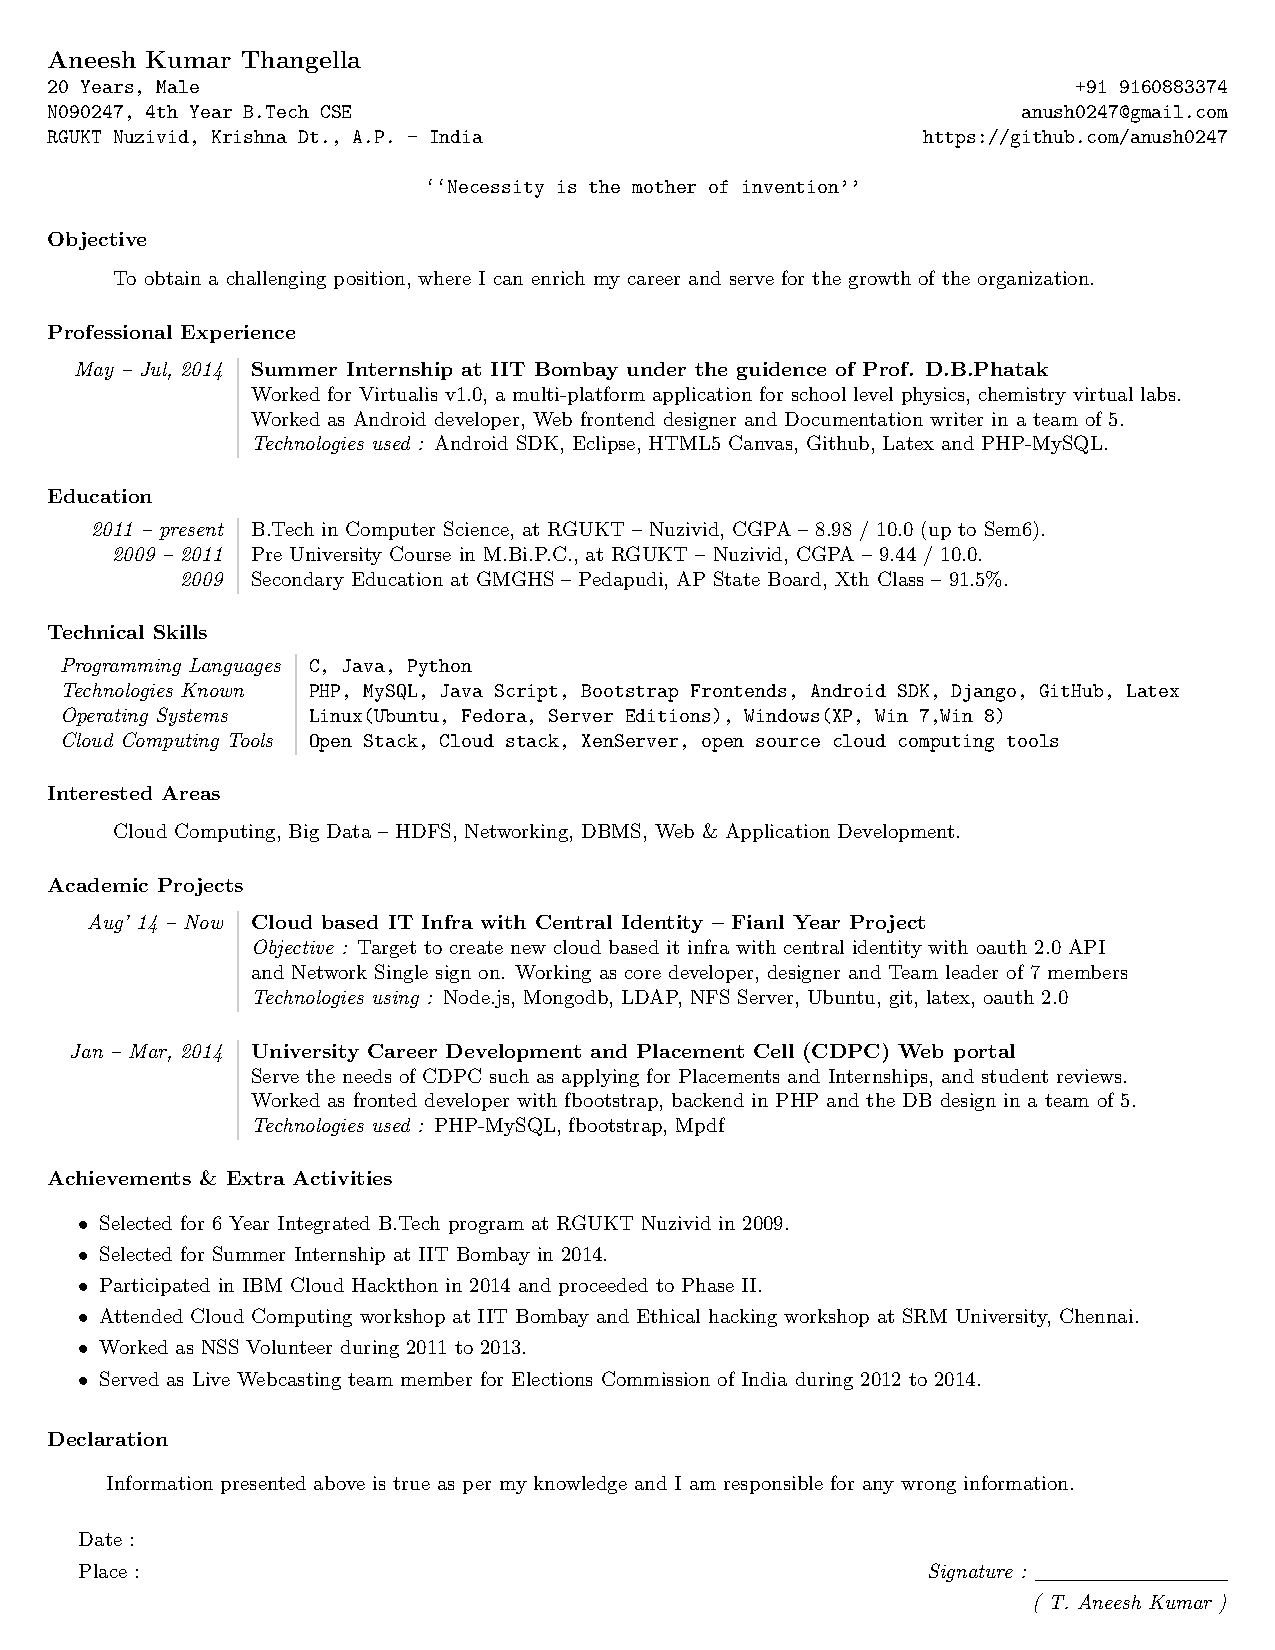
\includegraphics[width=2cm, height = 2.5cm]{aneesh.jpg}
%\end{flushright}

\end{flushright}
\end{multicols}


%\begin{center}
%\url{ ``Necessity is the mother of invention'' }
%\end{center} 

\subsubsection*{Objective}
\hspace{1cm} To obtain a challenging position, where I can enrich my career and serve for the growth of the organization.

\subsubsection*{Education}
\begin{tabular}{L!{\VRule}R}
\textit{2011 -- present} & B.Tech in Computer Science, at RGUKT -- Nuzvid, \textbf{CGPA -- 8.98 / 10.0} (till now).\\
\textit{2009 -- 2011 }&  Pre University Course in M.Bi.P.C., at RGUKT -- Nuzvid, \textbf{CGPA -- 9.44 / 10.0}.\\
\textit{2009 } &  Secondary Education at GMGHS -- Pedapudi, AP State  Board, \textbf{Xth Class -- 91.5\%.}\\
\end{tabular}



\subsubsection*{Professional Experience}
\begin{tabular}{L!{\VRule}R}
\textit{ May -- Jul, 2014}&{\bf Summer Internship at IIT Bombay under the guidence of Prof. D.B.Phatak} \\
& Worked for Virtualis v1.0, a multi-platform application for school physics, chemistry virtual labs. \\
& Worked as Android developer, Web frontend designer and Documentation writer in a team of 5. \\
& \textit{Technologies used :} Android SDK, Eclipse, HTML5 Canvas, Github, Latex and PHP-MySQL.\\
\end{tabular}

\subsubsection*{Technical Skills}
\begin{tabular}{l !{\VRule} R}
\textit{Programming Languages} &  \url{C, Java, Python, PHP, MySQL, Java Script }\\
\textit{Technologies Known}&	\url{Android SDK, Django, Node.js, GitHub, Latex, Bootstrap, Semantic UI} \\
\textit{Operating Systems} &	\url{Linux(Ubuntu, Fedora, Server Editions), Windows }\\
\textit{Cloud Computing Tools} 	&	\url{Open Stack, Cloud stack, XenServer, open source cloud computing tools} \\
\end{tabular}

\subsubsection*{Interested Areas of Working}
\begin{multicols}{2}
%\hspace{1cm} Cloud Computing, Big Data -- HDFS, Networking \& Databases, GUI Design, Web \& Application Development.
%\onehalfspacing
\begin{compactitem}
	\item Cloud Computing, Big Data -- HDFS
	\item Networking \& Databases 
	\item Frontend Design \& Development
	\item Web \& Application Development 
\end{compactitem}
%\begin{flushright}
%\underline{}
%\end{flushright}
\end{multicols}

\subsection*{Projects Contributed}

\begin{tabular}{L!{\VRule}R}
\textit{ Aug' 14 -- Now}&{\bf Cloud based IT Infra with Central Identity -- Final Year Project } \\
& \textit{Objective :} Target to create new cloud based it infra with central identity with oauth 2.0 API\\
& and Network Single sign on. Working as core developer, designer and Team leader of 7 members \\
& \textit{Technologies using:} Node.js, Mongodb, LDAP, NFS Server, Ubuntu, git, latex, oauth 2.0\\
& \textit{Github Repo : }\url{https://github.com/reboot14/rinfra/}\\
\end{tabular}
\newline \linebreak \\
\begin{tabular}{L!{\VRule}R}
\textit{ Dec' 14}&{\bf ChatBoard v0.1 -- Collaborative Class room Interaction Tool for Amazon Hackthon } \\
& Useful in digital class room interaction from teacher to students, can share common white board.\\
& Worked as Frontend developer with semantic-ui, backend in Node.js, socket.io and lead team of 3. \\
& \textit{Technologies used :} Node.js, Express.js, Sokcet.io, HTML5 Canvas, Semantic UI\\
& \textit{Github Repo : }\url{https://github.com/reboot14/hackthon/}\\
\end{tabular}
\newline \linebreak \\
\begin{tabular}{L!{\VRule}R}
\textit{ Jan -- Mar' 14}&{\bf University Career Development and Placement Cell (CDPC) Web portal} \\
& Serve the needs of CDPC such as applying for Placements and Internships, and student reviews.\\
& Worked as fronted developer with fbootstrap, backend in PHP and the DB design in a team of 5. \\
& \textit{Technologies used :} PHP-MySQL, fbootstrap, Mpdf\\
& \textit{Hosted at : }\url{http://rgukttnp.rgukt.in:8888/cdpc/}\\
\end{tabular}
\newline \linebreak \\
\begin{tabular}{L!{\VRule}R}
\textit{ Jun -- Aug' 13}&{\bf Departmental Online Attendance Portal} \\
& Serve the attendance related needs like end semester eligibility and monthly reports and statistics.\\
& Worked as fronted developer with Bootstrap, backend in PHP and the DB design in a team of 5. \\
& \textit{Technologies used :} PHP-MySQL, Bootstrap, Mpdf, Flash Charts for plotting daily submissions\\
\end{tabular}

\subsection*{Achievements }
%\begin{spacing}{onehalfspacing}
\onehalfspacing
\begin{compactitem}
	\item Selected for 6 years integrated B.Tech program at RGUKT Nuzvid in 2009.
	\item Selected for Summer Internship at \textbf{IIT Bombay} in 2014.
	\item Secured 2$ ^{nd} $ position in \textbf{Amazon Hackthon 2014} organized by Pragyan, NITT.
	\item Participated in \textbf{IBM Cloud Hackthon} in 2014 and qualified for phase II.
	\item Secured 1$^{st}$ position in CTF at TeckZite'14, Technical Fest at RGUKT - Nuzvid.
	%\item Secured campus top 50th rank in Internatioanl Maths Olympiad in 2010.  
\end{compactitem}
%\end{spacing}

\subsection*{Extra Academic Activities}
\onehalfspacing
\begin{compactitem}
	\item Organized one day workshop on cloud computing by Dept. of CSE \& Manjrasoft Pty Ltd. at RGUKT Nuzvid.
	\item Attended Cloud Computing workshop in TechFest'14 at IIT Bombay. 
	\item Attended Ethical hacking workshop in E-Hack'14 at SRM University, Chennai.
	%\item Presentation by me on Virtualization at RGUKT, Nuzvid in TechnoStart -2013.
	\item Worked as NSS volunteer during 2011 to 2013.
	\item Currently working in CSE Dept. Technical support team from 2013. 
	\item Served as Live Webcasting team member for 5 times to The Elections Commission of India during 2012 to 2014.
\end{compactitem}

\subsection*{Personal Assets}
\onehalfspacing
\begin{multicols}{2}
\begin{compactitem}
	\item Active team member and leader
	\item Quick Learning Ability
	\item Punctual \& Self obedient
%	\item Optimistic \& Enthusiastic
	\item Service minded \& Eco loving
\end{compactitem}
\end{multicols}

\begin{multicols}{2}

\subsection*{Personal Information}
\begin{tabular}{L!{\VRule}R}
\textit{ Father Name }& Mr. China Venkata Ramana\\
\textit{ Mother Name }& Mrs. Subbayyamma\\
%\textit{ Sisters Names }& Aruna Devi, Satya Gowri\\
\textit{ Date of Birth }& 06 Feb, 1994\\
\textit{ Languages}& English, Telugu\\
%\textit{ }& \\
\textit{Hobbies } & Listening to Music, Web surfing \\
%\textit{Religion } & Hindu
\end{tabular}

\begin{flushright}


\begin{flushleft}
\subsection*{Permanent Address}
\end{flushleft}

\begin{tabular}{L!{\VRule} R}
\textit{ D.No \& Street }& 5 - 73, New Gowri Devi Temple St.\\
\textit{ Village}& Pedapudi Village \\
%\textit{ Village  }& Pedapudi \\
\textit{ Mandal }& Pedapudi Mandal \\
\textit{ City \& Dist.  }& Kakinada, East Godavari Dist.\\
\textit{ State \& Country }& Andhra Pradesh, India -- 533006\\
%\textit{ Country  } & India -- 533006 \\
%\textit{ Pincode }& 533006
\end{tabular}

\end{flushright}


\end{multicols}


\subsection*{Declaration}
\hspace{1cm}Information presented above is true as per my knowledge and I am responsible for any wrong information.

\begin{multicols}{2}
 Date : \\
 \indent Place : 
\begin{flushright}
\underline{} \\
\textit{
 Signature : \underline{ \hspace{3cm} } \\
  ( T. Aneesh Kumar )
}
\end{flushright}
\end{multicols}

\end{document}